\documentclass[12pt,a4paper]{article}

% --- Пакеты ---
\usepackage[utf8]{inputenc}
\usepackage[T2A]{fontenc}
\usepackage[russian]{babel}
\usepackage{amsmath, amssymb, amsthm}
\usepackage{geometry}
\usepackage{graphicx}
\usepackage{hyperref}
\usepackage{enumitem}

\geometry{left=2.5cm, right=2cm, top=2cm, bottom=2cm}

% --- Теоремы и определения ---
\newtheorem{theorem}{Теорема}
\newtheorem{lemma}{Лемма}
\theoremstyle{definition}
\newtheorem{definition}{Определение}
\newtheorem{remark}{Замечание}

% --- Команды ---
\newcommand{\E}{E}
\newcommand{\R}{\mathbb{R}}
\newcommand{\Leb}{\int_{E}}
\newcommand{\LS}{\int_{E} f \, d\mu_F}
\newcommand{\muF}{\mu_F}

\begin{document}

% --- Шапка ---
\begin{center}
    {\Large \textbf{Лабораторная работа 4-1, Вариант 8}}\\[0.4em]
    {\normalsize Математический анализ, 4 семестр}\\[0.2em]
    {\normalsize Инютин Святослав \quad Группа: М3232}\\[0.2em]
    {\normalsize Дата: \today}
\end{center}
\vspace{1.5em}

\section*{Условие}

Дано:
\[
    f(x) = x^2, \quad E = [1,4], \quad F(x) = \sqrt{x}.
\]

\section{Аналитический метод}

% --- 1.1 ---
\subsection{Измеримость функции $f$ по Лебегу на $E$}

Сначала докажем, что множество $E = [1,4]$ измеримо по Лебегу.

\begin{lemma}[1.2.1]
    Любой брус $\langle a, b \rangle$ ($a_k, b_k \in \mathbb{R},\; k = 1, \ldots, n$)
    измерим по Лебегу и его мера равна классическому объёму ячейки с такими же концами:
    \[
        \lambda\langle a, b \rangle = \prod_{k=1}^{n}(b_k - a_k).
    \]
\end{lemma}

\begin{proof}
    По лемме 1.2.1: отрезок $[1,4]$ является замкнутым бруском
    с конечными концами $a=1$, $b=4$, следовательно $E=[1,4]$ измеримо
    по Лебегу и $\lambda(E) = 4 - 1 = 3$.
\end{proof}

Теперь докажем, что функция $f(x) = x^2$ измерима по Лебегу на $E$.

\begin{proof}
    По следствию 1.2.2 из рассматриваемой выше леммы: замкнутые множества измеримы по Лебегу.
    Для любого $c \in \R$ рассмотрим множество $\{x \in E : f(x) > c\}$:

    \begin{enumerate}
        \item Если $c < 1$: $\{x \in [1,4] : x^2 > c\} = [1,4]$ -- брус, измеримо.
        \item Если $c \geq 16$: $\{x \in [1,4] рассматриваемой: x^2 > c\} = \varnothing$ -- измеримо.
        \item Если $1 \leq c < 16$: $\{x \in [1,4] : x^2 > c\} = (\sqrt{c},\, 4]$ --
              брус (полуоткрытый отрезок), измеримо по лемме 1.2.1.
    \end{enumerate}

    Во всех случаях надлебежевское множество измеримо, следовательно $f$ измерима по Лебегу на $E$.
\end{proof}

% --- 1.2 ---
\subsection{Последовательность простых функций $f_n(x)$}

Построим последовательность простых функций $f_n(x) \leq f(x)$, $f_n \to f$ почти всюду на $E$,
начиная с $f_0(x) = 0$.

Разобьём $E = [1,4]$ на $n$ равных частей:
\[
    x_k^{(n)} = 1 + \frac{3k}{n}, \quad k = 0, 1, \ldots, n,
    \quad \Delta x = \frac{3}{n}.
\]

Определим:
\[
    f_n(x) = \sum_{k=0}^{n-1} f\!\left(x_k^{(n)}\right) \cdot \mathbf{1}_{[x_k^{(n)},\, x_{k+1}^{(n)})}(x)
    = \sum_{k=0}^{n-1} \left(1 + \frac{3k}{n}\right)^2
      \cdot \mathbf{1}_{\left[1+\frac{3k}{n},\, 1+\frac{3(k+1)}{n}\right)}(x).
\]

\textbf{Свойства:}
\begin{enumerate}
    \item \textbf{Начальное условие:} $f_0(x) = 0$ для всех $x \in E$.
    \item \textbf{Оценка снизу:} $f_n(x) \leq f(x)$ на $E$, так как $f(x) = x^2$ не убывает
          на $[1,4]$, а на каждом отрезке $[x_k^{(n)}, x_{k+1}^{(n)})$ берётся значение в
          левом конце: $f_n(x) = f(x_k^{(n)}) \leq f(x)$.
    \item \textbf{Поточечная сходимость:} для любого $x \in E$ и достаточно большого $n$
          найдётся $k$ такое, что $x \in [x_k^{(n)}, x_{k+1}^{(n)})$, и тогда
          $|f_n(x) - f(x)| = f(x) - f(x_k^{(n)}) \leq f'(\xi)\cdot\frac{3}{n} \to 0$.
          Следовательно $f_n \to f$ поточечно, а значит и почти всюду на $E$.
\end{enumerate}

% --- 1.3 ---
\subsection{Сходимость интегралов Лебега}

\begin{theorem}[Леви о монотонной сходимости]
    Если $0 \leq f_n$ возрастает $f$ почти всюду на $E$ и $f_n$ измеримы, то
    \[
        \lim_{n \to \infty} \int_E f_n \, d\mu = \int_E f \, d\mu.
    \]
\end{theorem}

Так как последовательность $\{f_n\}$ монотонно не убывает $f_n \leq f_{n+1}$, и при
измельчении разбиения значения на каждом подотрезке не уменьшаются и $f_n \to f$
на $E$. Все $f_n$ неотрицательны и измеримы как простые функции. Следовательно теореме Леви:
\[
    \lim_{n \to \infty} \int_E f_n \, d\mu = \int_E f \, d\mu = \int_1^4 x^2 \, dx.
\]

Вычислим интеграл Лебега:
\[
    \int_E f \, d\mu = \int_1^4 x^2 \, dx
    = \left[\frac{x^3}{3}\right]_1^4
    = \frac{64}{3} - \frac{1}{3} = \frac{63}{3} = 21.
\]

% --- 1.4 ---
\subsection{Мера Лебега–Стилтьеса $\mu_F$}

Покажем, что $F(x) = \sqrt{x}$ задаёт меру Лебега–Стилтьеса $\mu_F$.

\begin{proof}
    Функция $F$ задаёт меру Лебега–Стилтьеса тогда и только тогда, когда она
    монотонно не убывает и непрерывна справа.
    \begin{enumerate}
        \item \textbf{Монотонность:} $F'(x) = \dfrac{1}{2\sqrt{x}} > 0$ при $x > 0$,
              следовательно $F$ строго возрастает на $(0,+\infty)$, в частности на $[1,4]$.
        \item \textbf{Непрерывность справа:} $F(x) = \sqrt{x}$ непрерывна на $(0, +\infty)$
              (как элементарная функция), поэтому непрерывна справа в каждой точке.
    \end{enumerate}
    Следовательно $F$ порождает меру Лебега–Стилтьеса $\mu_F$ на $(\mathbb{R}, \mathcal{B}(\mathbb{R}))$,
    причём $\mu_F\bigl((a,b]\bigr) = F(b) - F(a) = \sqrt{b} - \sqrt{a}$.
\end{proof}

% --- 1.5 ---
\subsection{Интеграл Лебега–Стилтьеса}

Поскольку $F(x) = \sqrt{x}$ непрерывна и дифференцируема на $E = [1,4]$, интеграл
Лебега–Стилтьеса сводится к интегралу Римана:
\[
    \int_E f \, d\mu_F = \int_1^4 f(x) \, dF(x) = \int_1^4 x^2 \cdot F'(x) \, dx
    = \int_1^4 x^2 \cdot \frac{1}{2\sqrt{x}} \, dx.
\]

Упростим подынтегральное выражение:
\[
    x^2 \cdot \frac{1}{2\sqrt{x}} = \frac{x^2}{2x^{1/2}} = \frac{x^{3/2}}{2}.
\]

Вычислим:
\[
    \int_E f \, d\mu_F = \int_1^4 \frac{x^{3/2}}{2} \, dx
    = \frac{1}{2} \cdot \left[\frac{x^{5/2}}{5/2}\right]_1^4
    = \frac{1}{2} \cdot \frac{2}{5} \left[x^{5/2}\right]_1^4
    = \frac{1}{5} \left(4^{5/2} - 1^{5/2}\right).
\]

Так как $4^{5/2} = (2^2)^{5/2} = 2^5 = 32,$ то:
\[
    \int_E f \, d\mu_F = \frac{1}{5}(32 - 1) = \frac{31}{5} = 6{,}2.
\]

\section{Численный метод}

\subsection{Графики $f_n(x)$}

\begin{figure}[h!]
    \centering
    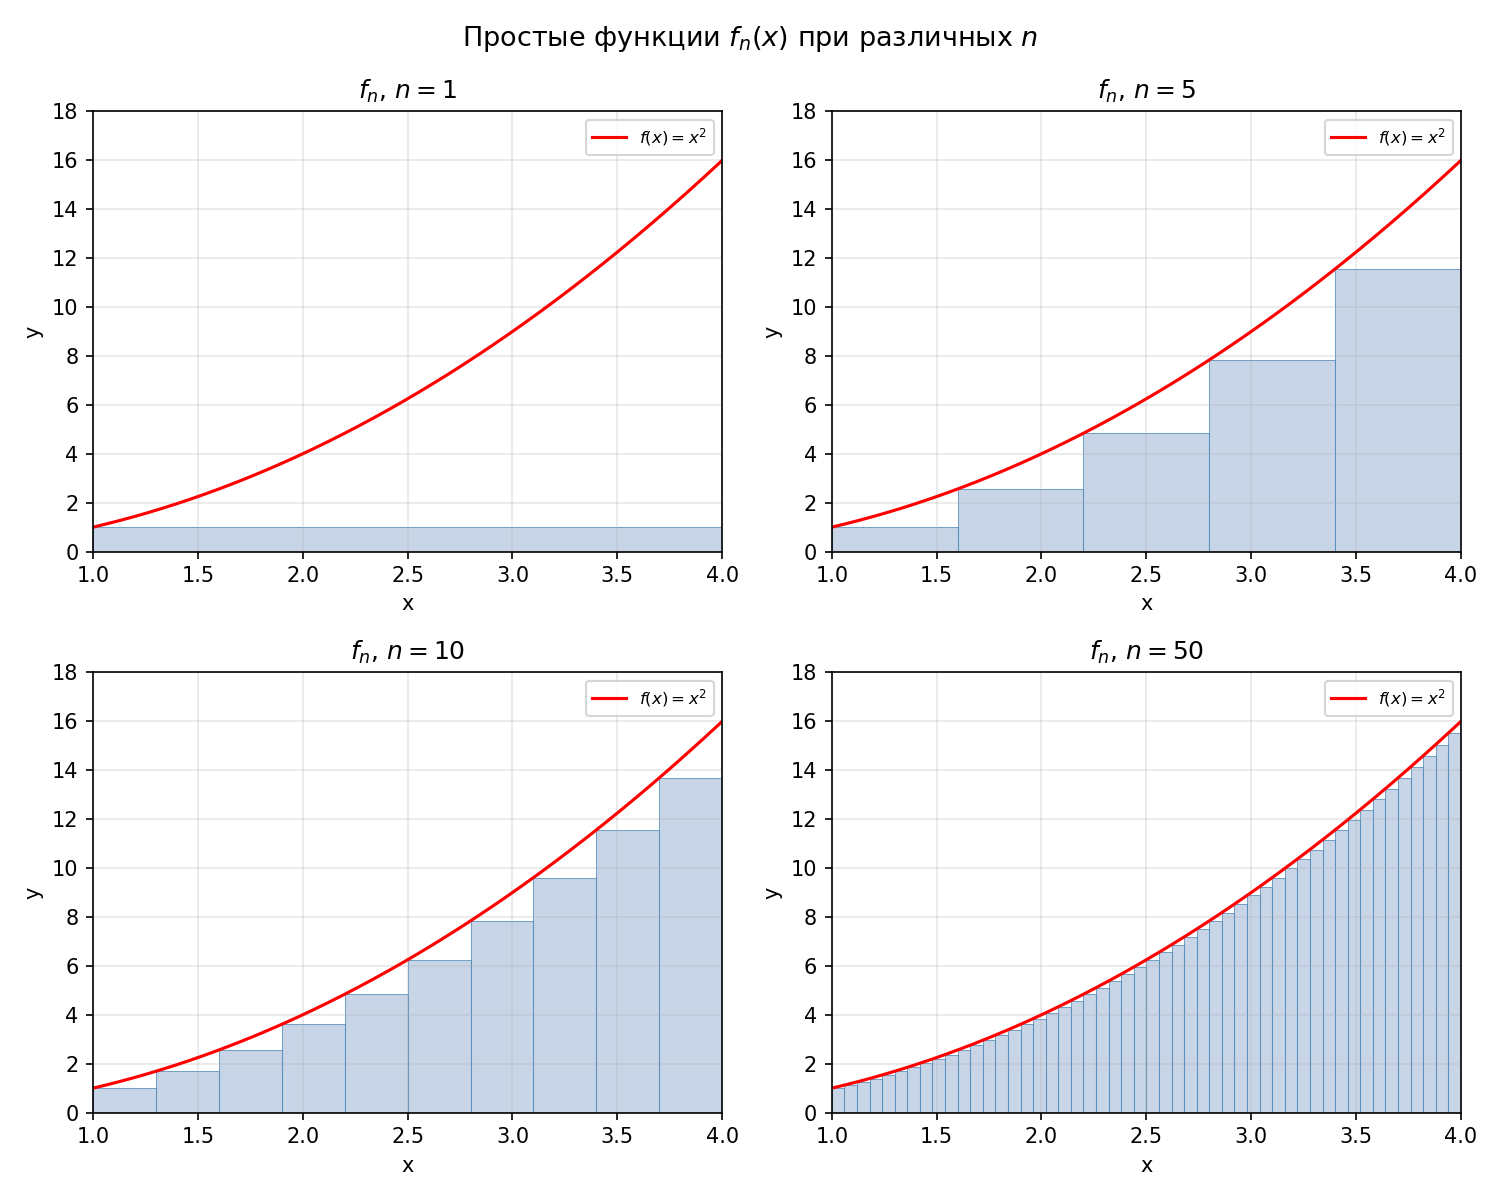
\includegraphics[width=0.8\textwidth]{graphs.png}
    \caption{Графики простых функций $f_n(x)$ при различных $n$}
\end{figure}

\subsection{Интеграл Лебега от \texorpdfstring{$f_n$}{f\_n}}

Интеграл Лебега от простой функции $f_n$ вычисляется как:
\[
    \int_E f_n \, d\mu = \sum_{k=0}^{n-1} \left(1 + \frac{3k}{n}\right)^2 \cdot \frac{3}{n}.
\]

\begin{center}
\begin{tabular}{|c|c|c|}
    \hline
    $n$ & $\displaystyle\int_E f_n \, d\mu$ & Погрешность \\
    \hline
    10   & $18{,}79500000$ & $2{,}21 \cdot 10^{0}$ \\
    100  & $20{,}77545000$ & $2{,}25 \cdot 10^{-1}$ \\
    1000 & $20{,}97750450$ & $2{,}25 \cdot 10^{-2}$ \\
    \hline
    $\infty$ (аналит.) & $21$ & $0$ \\
    \hline
\end{tabular}
\end{center}

\subsection{Интеграл Лебега–Стилтьеса от \texorpdfstring{$f_n$}{f\_n}}

\[
    \int_E f_n \, d\mu_F = \sum_{k=0}^{n-1} \left(1 + \frac{3k}{n}\right)^2
    \cdot \left(\sqrt{1 + \frac{3(k+1)}{n}} - \sqrt{1 + \frac{3k}{n}}\right).
\]

\begin{center}
\begin{tabular}{|c|c|c|}
    \hline
    $n$ & $\displaystyle\int_E f_n \, d\mu_F$ & Погрешность \\
    \hline
    50   & $6{,}06089551$ & $1{,}39 \cdot 10^{-1}$ \\
    500  & $6{,}18600900$ & $1{,}40 \cdot 10^{-2}$ \\
    5000 & $6{,}19860009$ & $1{,}40 \cdot 10^{-3}$ \\
    \hline
    $\infty$ (аналит.) & $31/5 = 6.2$ & $0$ \\
    \hline
\end{tabular}
\end{center}

\subsection{Выводы}

\begin{enumerate}
    \item Последовательность $f_n \to f$ монотонно снизу, поэтому интегралы от $f_n$
          сходятся к аналитическому значению снизу.
    \item С ростом $n$ погрешность убывает как $O(1/n)$, что соответствует
          скорости сходимости суммы Римана.
    \item Значение интеграла Лебега: $\displaystyle\int_E x^2 \, d\mu = 21$.
    \item Значение интеграла Лебега–Стилтьеса: $\displaystyle\int_E x^2 \, d\mu_F = \frac{31}{5}$.
    \item Время работы программы: \texttt{0.0029} сек.
\end{enumerate}

\end{document}